\chapter{Bildvorverarbeitung}
Die Bildvorverarbeitung stellt ein essenziellen Schritt zur Lokalisierung der \QRCodes dar. Das Eingabebild wird in dieser Phase zuerst in ein Graustufenbild umgewandelt und danach binarisiert. Der Einfachheit halber werden zu große Bilder zuerst noch auf unter 1500 in der größten Dimension verkleinert. \OpenCV bietet die Möglichkeit Bilder direkt als Graustufenbild einzulesen, welches für Schwellenwertoperationen genutzt wird.
Die Klasse \texttt{ImageBinarization} ist für die darauf folgende Binarisierung zuständig. 
\inputCPP[label={lst:binarize}][][Ablauf der Binarisierung.]{code/binarize-run.cpp}

In Zeile 4 wird die Methode \texttt{computeSmoothing} aufgerufen, die eine Gaußglättung auf dem Bild durchführt, um den Einfluss von Rauschen zu mindern. Um mit verschiedenen Belichtungsszenarien umgehen zu können, sind drei Methoden zur Schwellwertberechnung implementiert:
\begin{itemize}
	\item Globales Schwellwertverfahren
	\item Mittelwert-Schwellwertverfahren
	\item Gaußsches-Schwellwertverfahren
\end{itemize}
\inputCPP[label={lst:globalthreshold}][][Binarisierung anhand des globalen Schwellwertverfahrens.]{code/global-binarize.cpp}
Im ersten Durchlauf wird das globale Schwellwertverfahren angewandt. Bei der Berechnung wird auf die \texttt{threshold} Methode, wie sie im Listing \ref{lst:globalthreshold} steht, zurückgegriffen. Diese verwendet den \emph{Otsu} Algorithmus\footnote{Mehr Information zu dem Algorithmus auf der zugehörigen \OpenCV Seite:\url{http://docs.opencv.org/2.4/modules/imgproc/doc/miscellaneous_transformations.html\#threshold}}, um einen globalen Schwellwert zu berechnen und dann das Bild zu binarisieren.

Sollte mit dieser Methode im späteren Verlauf nicht mindestens drei \fps lokalisiert werden, wird das nächste Verfahren ausgeführt.

\inputCPP[label={lst:localthreshold}][][Binarisierung anhand eines lokalen Schwellwertverfahrens.]{code/local-binarize.cpp}

Bei den lokalen Schwellwertverfahren wird die Methode \texttt{adaptiveThreshold} verwendet, welche in Listing \ref{lst:localthreshold} veranschaulicht wird. Im Gegensatz zum globalen Schwellwertverfahren, wird hier für jeden Pixel anhand der Nachbarschaft ein eigener Schwellwert errechnet. Als empirisch gut geeignet hat sich eine Nachbarschaft von $11 \times 11$ herausgestellt.

Die Berechnung des Schwellwerts für die Nachbarschaft erfolgt auf zwei unterschiedliche Verfahren:
\begin{description}
	\item[\texttt{ADAPTIVE\_THRESH\_MEAN\_C}:] Der Mittelwert der Nachbarschaft.
	\item[\texttt{ADAPTIVE\_THRESH\_GAUSSIAN\_C}:] Ein Gauß gewichteter Mittelwert der Nachbarschaft.
\end{description}

Der Parameter \texttt{C} wird vom Mittelwert subtrahiert. In der Implementierung wird \texttt{C} konstant $0$ gewählt.

\begin{figure}[h]
\centering
\begin{subfigure}[t]{0.48\textwidth}
\centering
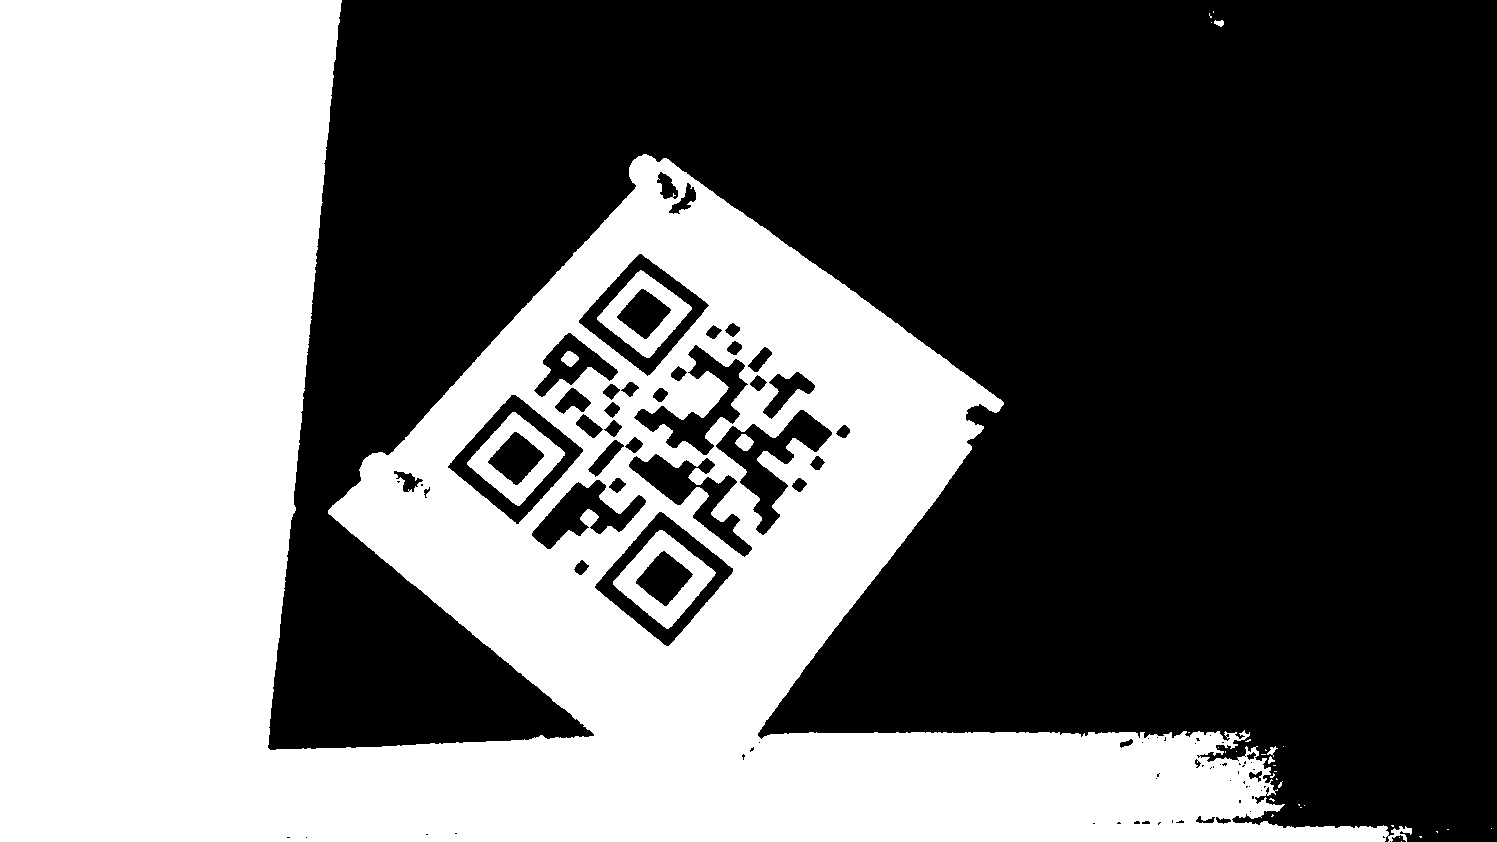
\includegraphics[scale=0.12]{images/qrcode-adler-wand_1___BINARIZED___.jpg}
\caption{globales Schwellwertverfahren}
\end{subfigure}%
\begin{subfigure}[t]{0.48\textwidth}
\centering
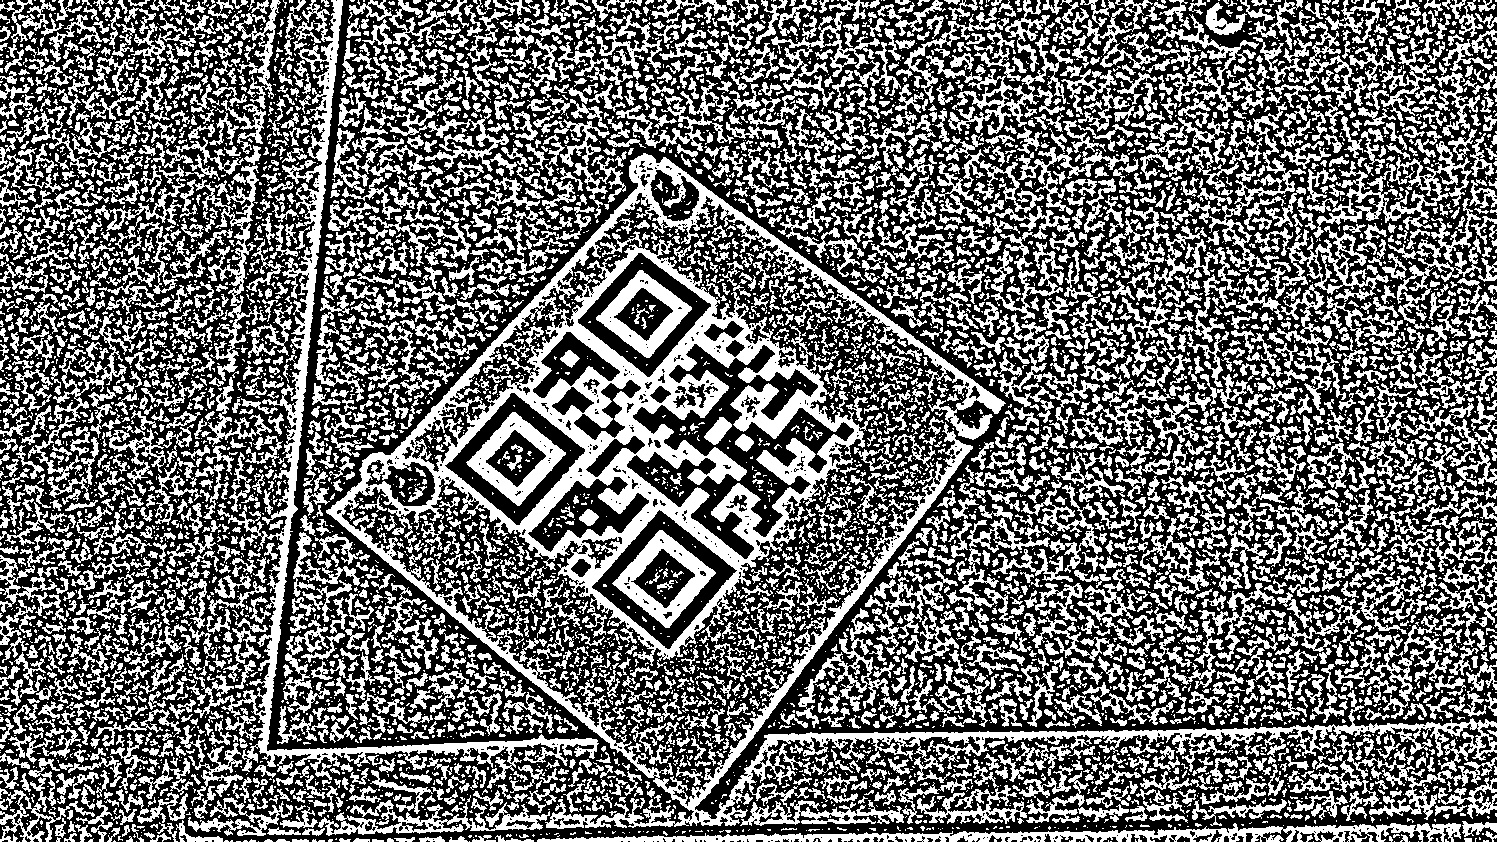
\includegraphics[scale=0.12]{images/qrcode-adler-wand_2___BINARIZED___.jpg}
\caption{lokales Schwellwertverfahren}
\end{subfigure}
\caption{Das Resultat der Binarisierung mit den jeweiligen Verfahren. Links global und Rechts lokal.}
\end{figure}